\documentclass[9pt]{article}
\usepackage[sc,osf]{mathpazo}   % With old-style figures and real smallcaps.
\linespread{1.025}              % Palatino leads a little more leading
% Euler for math and numbers
\usepackage[euler-digits,small]{eulervm}
\usepackage{amsmath}
\usepackage{amssymb}
\usepackage{physics}
\usepackage{tikz}
\usepackage{fancyhdr}
\author{Siddharth Bhat(20161105)}
\title{Optimization assignment --- Bala's algorithm 4}
\date{\today}

\pagestyle{fancy}
\fancyhf{}
\lhead{Siddharth Bhat (20161105)}
\rfoot{Page \thepage}

\begin{document}
\maketitle
\thispagestyle{fancy}
\begin{align*}
    \min: -15x_1 -25x_2 -12x_3 -10x_4 \qquad 
    1: 3x_1 + 6x_2 + 5x_3 + 5x_4 \leq 12 ;~
    2: 4x_2 + 9x_2 - 2x_3 + x_4 \leq 25
\end{align*}
\begin{itemize}
    \item Branch on $x_1$. Both solutions feasible. Branch on smaller
        tentative solution $x_1 = 0$.
    \item Branch on $x_2$. Both solutions are feasible. Branch on smaller
        tentative solution $x_2 = 1$

    \item Branch of $x_3$. Both solutions are feasible. Branch on smaller
        tentative solution $x_3 = 1$.
\end{itemize}
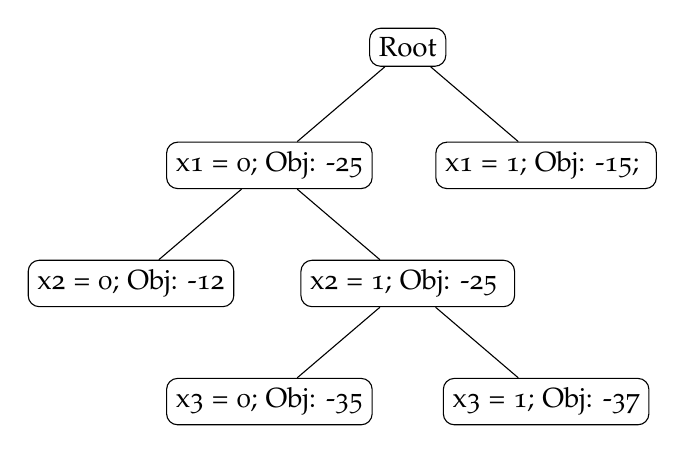
\begin{tikzpicture}[sibling distance=10em,
  every node/.style = {shape=rectangle, rounded corners,
  draw, align=center}]]
  \node {Root}
      % x1 = 0
      child { 
          node{x1 = 0; Obj: -25}
          % x2 = 0
          child { node {x2 = 0; Obj: -12} }
          % x2 = 1
          child { node {x2 = 1; Obj: -25 } 
              % x3 = 0
              child { node {x3 = 0; Obj: -35}}
              % x3 = 1
              child { node {x3 = 1; Obj: -37}}
              }
          }
      % x1 = 1
      child {node{x1 = 1; Obj: -15; } };
  %\node {Formulas}
  %  child { node {single-line} }
  %  child { node {multi-line}
  %    child { node {aligned at}
  %      child { node {relation sign} }
  %      child { node {several places} }
  %      child { node {center} } }
  %    child { node {first left,\\centered,\\last right} } };
\end{tikzpicture}
\end{document}

